\documentclass[11pt,a4paper]{article}
\usepackage[margin=2cm]{geometry}
\usepackage{graphicx}
\usepackage{tabularx}
\usepackage{booktabs}
\usepackage{xcolor}
\usepackage{fancyhdr}
\usepackage{listings}
\usepackage{tikz}
\usetikzlibrary{shapes,arrows,positioning}
\usepackage{amsmath}
\usepackage{hyperref}

% Define colors
\definecolor{headercolor}{RGB}{25,25,112}
\definecolor{sectioncolor}{RGB}{70,130,180}
\definecolor{codebackground}{RGB}{245,245,245}

% Header and footer
\pagestyle{fancy}
\fancyhf{}
\fancyhead[L]{\textcolor{headercolor}{\textbf{RISC-V RV32I Pipelined Processor}}}
\fancyhead[R]{\textcolor{headercolor}{\textbf{Datasheet v1.0}}}
\fancyfoot[C]{\thepage}

% Code listing style
\lstset{
    backgroundcolor=\color{codebackground},
    basicstyle=\footnotesize\ttfamily,
    breaklines=true,
    frame=single,
    language=Verilog
}

\begin{document}

% Title Page
\begin{titlepage}
    \centering
    \vspace*{2cm}
    
    {\Huge\textbf{\textcolor{headercolor}{RISC-V RV32I}}}\\
    \vspace{0.5cm}
    {\LARGE\textbf{\textcolor{sectioncolor}{Pipelined Processor}}}\\
    \vspace{1cm}
    {\Large Technical Datasheet}\\
    \vspace{2cm}
    
    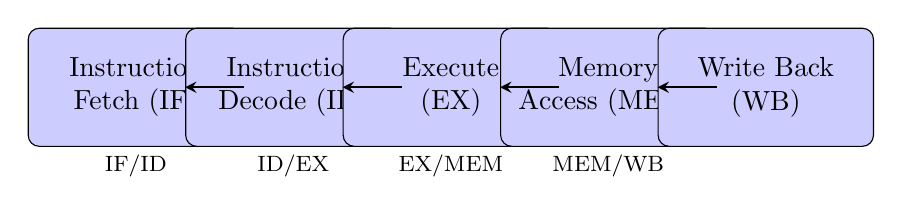
\begin{tikzpicture}[node distance=2cm, auto]
        % Define styles
        \tikzstyle{stage} = [rectangle, draw, fill=blue!20, text width=2.5cm, text centered, rounded corners, minimum height=1.5cm]
        \tikzstyle{arrow} = [thick,->,>=stealth]
        
        % Pipeline stages
        \node [stage] (if) {Instruction\\Fetch (IF)};
        \node [stage, right of=if] (id) {Instruction\\Decode (ID)};
        \node [stage, right of=id] (ex) {Execute\\(EX)};
        \node [stage, right of=ex] (mem) {Memory\\Access (MEM)};
        \node [stage, right of=mem] (wb) {Write Back\\(WB)};
        
        % Arrows
        \draw [arrow] (if) -- (id);
        \draw [arrow] (id) -- (ex);
        \draw [arrow] (ex) -- (mem);
        \draw [arrow] (mem) -- (wb);
        
        % Pipeline registers
        \node [below of=if, node distance=1cm] {\footnotesize IF/ID};
        \node [below of=id, node distance=1cm] {\footnotesize ID/EX};
        \node [below of=ex, node distance=1cm] {\footnotesize EX/MEM};
        \node [below of=mem, node distance=1cm] {\footnotesize MEM/WB};
    \end{tikzpicture}
    
    \vspace{2cm}
    {\large Version 1.0}\\
    \vspace{0.5cm}
    {\large \today}\\
    
    \vfill
    {\large Advanced Digital Systems Design}
\end{titlepage}

\tableofcontents
\newpage

\section{Overview}

\subsection{Introduction}
The RISC-V RV32I Pipelined Processor is a 32-bit processor implementation based on the RISC-V instruction set architecture. This design implements a classic 5-stage pipeline with advanced features including branch prediction, hazard detection, and data forwarding to achieve high performance while maintaining compatibility with the RV32I base integer instruction set.

\subsection{Key Features}
\begin{itemize}
    \item 32-bit RISC-V RV32I instruction set architecture
    \item 5-stage pipeline (IF, ID, EX, MEM, WB)
    \item Branch prediction for improved performance
    \item Data forwarding to minimize pipeline stalls
    \item Hazard detection and handling
    \item 32 × 32-bit general-purpose registers
    \item Support for all RV32I base instructions
    \item Synthesizable Verilog HDL implementation
\end{itemize}

\subsection{Applications}
\begin{itemize}
    \item Educational processor for computer architecture studies
    \item Embedded system applications
    \item FPGA-based system implementations
    \item Research and development platform
    \item Custom processor applications
\end{itemize}

\section{Architecture}

\subsection{Pipeline Overview}
The processor implements a classic 5-stage RISC pipeline:

\begin{table}[h]
\centering
\begin{tabularx}{\textwidth}{|l|X|}
\hline
\textbf{Stage} & \textbf{Function} \\
\hline
IF (Instruction Fetch) & Fetches instructions from memory, manages program counter \\
\hline
ID (Instruction Decode) & Decodes instructions, reads register file, generates control signals \\
\hline
EX (Execute) & Performs arithmetic/logic operations, calculates branch targets \\
\hline
MEM (Memory Access) & Handles load/store operations, accesses data memory \\
\hline
WB (Write Back) & Writes results back to register file \\
\hline
\end{tabularx}
\caption{Pipeline Stage Functions}
\end{table}

\subsection{Block Diagram}

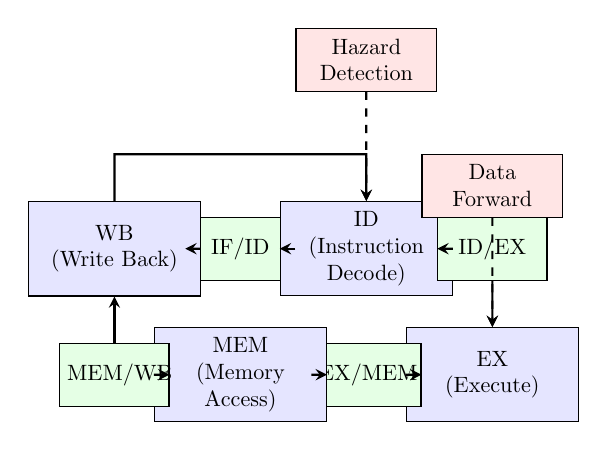
\begin{tikzpicture}[node distance=3cm, auto, scale=0.8, transform shape]
    % Define styles
    \tikzstyle{module} = [rectangle, draw, fill=blue!10, text width=2.5cm, text centered, minimum height=1.5cm]
    \tikzstyle{register} = [rectangle, draw, fill=green!10, text width=1.5cm, text centered, minimum height=1cm]
    \tikzstyle{control} = [rectangle, draw, fill=red!10, text width=2cm, text centered, minimum height=1cm]
    \tikzstyle{arrow} = [thick,->,>=stealth]
    
    % Main pipeline modules
    \node [module] (if) {IF\\(Instruction\\Fetch)};
    \node [register, right of=if, node distance=2cm] (ifid) {IF/ID};
    \node [module, right of=ifid, node distance=2cm] (id) {ID\\(Instruction\\Decode)};
    \node [register, right of=id, node distance=2cm] (idex) {ID/EX};
    \node [module, below of=idex, node distance=2cm] (ex) {EX\\(Execute)};
    \node [register, left of=ex, node distance=2cm] (exmem) {EX/MEM};
    \node [module, left of=exmem, node distance=2cm] (mem) {MEM\\(Memory\\Access)};
    \node [register, left of=mem, node distance=2cm] (memwb) {MEM/WB};
    \node [module, above of=memwb, node distance=2cm] (wb) {WB\\(Write Back)};
    
    % Control units
    \node [control, above of=id, node distance=3cm] (hazard) {Hazard\\Detection};
    \node [control, above of=ex, node distance=3cm] (forward) {Data\\Forward};
    
    % Arrows
    \draw [arrow] (if) -- (ifid);
    \draw [arrow] (ifid) -- (id);
    \draw [arrow] (id) -- (idex);
    \draw [arrow] (idex) -- (ex);
    \draw [arrow] (ex) -- (exmem);
    \draw [arrow] (exmem) -- (mem);
    \draw [arrow] (mem) -- (memwb);
    \draw [arrow] (memwb) -- (wb);
    \draw [arrow] (wb) -- ++(0,1.5) -| (id);
    
    % Control connections
    \draw [arrow, dashed] (hazard) -- (id);
    \draw [arrow, dashed] (forward) -- (ex);
\end{tikzpicture}

\section{Functional Specifications}

\subsection{Instruction Set Support}
The processor supports the complete RV32I base instruction set:

\begin{table}[h]
\centering
\begin{tabularx}{\textwidth}{|l|l|X|}
\hline
\textbf{Category} & \textbf{Instructions} & \textbf{Description} \\
\hline
Arithmetic & ADD, SUB, ADDI & Addition and subtraction operations \\
\hline
Logical & AND, OR, XOR, ANDI, ORI, XORI & Bitwise logical operations \\
\hline
Shift & SLL, SRL, SRA, SLLI, SRLI, SRAI & Left and right shift operations \\
\hline
Compare & SLT, SLTU, SLTI, SLTIU & Set-less-than operations \\
\hline
Branch & BEQ, BNE, BLT, BGE, BLTU, BGEU & Conditional branch instructions \\
\hline
Jump & JAL, JALR & Unconditional jump instructions \\
\hline
Load & LB, LH, LW, LBU, LHU & Load from memory instructions \\
\hline
Store & SB, SH, SW & Store to memory instructions \\
\hline
Upper Immediate & LUI, AUIPC & Upper immediate operations \\
\hline
\end{tabularx}
\caption{Supported RV32I Instructions}
\end{table}

\subsection{Register File}
\begin{itemize}
    \item 32 general-purpose registers (x0-x31)
    \item 32-bit register width
    \item x0 is hardwired to zero
    \item Dual-port read, single-port write
    \item Synchronous write, asynchronous read
\end{itemize}

\subsection{Memory Interface}
\begin{itemize}
    \item 32-bit address space
    \item Byte-addressable memory
    \item Support for 8-bit, 16-bit, and 32-bit memory operations
    \item Separate instruction and data memory interfaces
    \item Memory-mapped I/O support
\end{itemize}

\section{Performance Characteristics}

\subsection{Pipeline Performance}
\begin{table}[h]
\centering
\begin{tabular}{|l|l|}
\hline
\textbf{Parameter} & \textbf{Value} \\
\hline
Pipeline Depth & 5 stages \\
\hline
Theoretical CPI & 1.0 \\
\hline
Branch Penalty & 1-2 cycles (with prediction) \\
\hline
Load-Use Penalty & 1 cycle \\
\hline
Maximum Clock Frequency & Design dependent \\
\hline
\end{tabular}
\caption{Pipeline Performance Parameters}
\end{table}

\subsection{Hazard Handling}
\begin{itemize}
    \item \textbf{Data Hazards}: Resolved through data forwarding and pipeline stalling
    \item \textbf{Control Hazards}: Mitigated using branch prediction and early branch resolution
    \item \textbf{Structural Hazards}: Avoided through proper pipeline design
\end{itemize}

\section{Interface Specifications}

\subsection{Top-Level Module Interface}

\begin{lstlisting}[caption=TOP\_Pipelined\_design Module Interface]
module TOP_Pipelined_design #(parameter size = 32)(
    // Clock and Reset
    input clk,
    input reset,
    
    // Instruction Memory Interface
    input [size-1:0] instruction_i,
    output [size-1:0] ins_address,
    
    // Data Memory Interface
    input [size-1:0] MEM_result_i,
    output [size-1:0] RAM_DATA_o,
    output [size-1:0] RAM_Addr_o,
    output [2:0] RAM_DATA_control,
    output RAM_rw
);
\end{lstlisting}

\subsection{Signal Descriptions}

\begin{table}[h]
\centering
\begin{tabularx}{\textwidth}{|l|l|X|}
\hline
\textbf{Signal} & \textbf{Direction} & \textbf{Description} \\
\hline
clk & Input & System clock signal \\
\hline
reset & Input & Asynchronous reset (active high) \\
\hline
instruction\_i & Input & 32-bit instruction from instruction memory \\
\hline
ins\_address & Output & Instruction memory address \\
\hline
MEM\_result\_i & Input & Data from data memory (for loads) \\
\hline
RAM\_DATA\_o & Output & Data to be written to memory (for stores) \\
\hline
RAM\_Addr\_o & Output & Data memory address \\
\hline
RAM\_DATA\_control & Output & Memory operation control (byte/half/word) \\
\hline
RAM\_rw & Output & Memory read/write control \\
\hline
\end{tabularx}
\caption{Top-Level Signal Descriptions}
\end{table}

\section{Design Implementation}

\subsection{File Organization}
The design is organized in a hierarchical structure:

\begin{itemize}
    \item \textbf{digital\_top/}: Top-level integration module
    \item \textbf{instruction\_fetch/}: IF stage components
    \item \textbf{instruction\_decode/}: ID stage components  
    \item \textbf{execute/}: EX stage components
    \item \textbf{mem/}: MEM stage components
    \item \textbf{write\_back/}: WB stage components
    \item \textbf{pipeline\_register/}: Inter-stage registers
    \item \textbf{hazard/}: Hazard detection and forwarding
    \item \textbf{common/}: Shared utility modules
    \item \textbf{testbench/}: Verification components
\end{itemize}

\subsection{Key Components}

\subsubsection{Program Counter (PC\_new.v)}
Enhanced program counter with:
\begin{itemize}
    \item Branch prediction support
    \item JALR instruction handling
    \item Pipeline stall capability
    \item Misprediction correction
\end{itemize}

\subsubsection{Functional Unit (FU.v)}
Main execution unit containing:
\begin{itemize}
    \item Arithmetic unit for ADD/SUB operations
    \item Logic unit for bitwise operations
    \item Shifter for shift operations
    \item Comparison logic
\end{itemize}

\subsubsection{Data Forwarding Unit}
Handles data hazards by:
\begin{itemize}
    \item Detecting register dependencies
    \item Providing bypass paths
    \item Controlling multiplexer selection
\end{itemize}

\section{Timing Specifications}

\subsection{Clock Requirements}
\begin{itemize}
    \item Minimum clock period: Technology dependent
    \item Clock duty cycle: 50\% ± 5\%
    \item Clock skew: < 10\% of clock period
    \item Setup time: Technology dependent
    \item Hold time: Technology dependent
\end{itemize}

\subsection{Reset Specifications}
\begin{itemize}
    \item Reset type: Asynchronous assert, synchronous deassert
    \item Reset duration: Minimum 2 clock cycles
    \item Reset recovery time: 1 clock cycle after deassertion
\end{itemize}

\section{Power Specifications}

\subsection{Power Consumption}
Power consumption varies based on:
\begin{itemize}
    \item Clock frequency
    \item Activity factor
    \item Technology node
    \item Supply voltage
    \item Temperature
\end{itemize}

\subsection{Power Management}
\begin{itemize}
    \item Clock gating for unused modules
    \item Pipeline bubbling to reduce activity
    \item Optional low-power modes
\end{itemize}

\section{Verification and Testing}

\subsection{Testbench Coverage}
The design includes comprehensive testbenches:

\begin{table}[h]
\centering
\begin{tabularx}{\textwidth}{|l|X|}
\hline
\textbf{Testbench} & \textbf{Purpose} \\
\hline
Pipeline\_tb.v & Complete processor functionality testing \\
\hline
RegisterFile\_tb.v & Register file read/write operations \\
\hline
PC\_tb.v & Program counter functionality \\
\hline
Controller\_tb.v & Control unit verification \\
\hline
Datapath\_tb.v & Datapath component testing \\
\hline
NVRAM\_tb.v & Memory interface verification \\
\hline
\end{tabularx}
\caption{Testbench Components}
\end{table}

\subsection{Test Programs}
Specialized test programs verify:
\begin{itemize}
    \item Basic instruction functionality
    \item Branch and jump operations
    \item Load/store operations
    \item Pipeline hazard handling
    \item Forwarding mechanisms
\end{itemize}

\section{Synthesis and Implementation}

\subsection{Synthesis Requirements}
\begin{itemize}
    \item Verilog-2001 compliant code
    \item Synthesizable constructs only
    \item No behavioral delays in synthesizable code
    \item Proper reset handling
\end{itemize}

\subsection{Resource Utilization}
Typical resource requirements (technology dependent):
\begin{itemize}
    \item Logic cells: Moderate complexity
    \item Memory blocks: For register file implementation
    \item DSP blocks: Not required
    \item I/O pins: Configurable based on memory interface
\end{itemize}

\section{Application Notes}

\subsection{Memory System Integration}
\begin{itemize}
    \item Instruction and data memories can be separate or unified
    \item Memory latency affects pipeline performance
    \item Cache integration possible for improved performance
    \item Memory-mapped I/O supported
\end{itemize}

\subsection{Debug and Trace}
\begin{itemize}
    \item Internal signals accessible for debugging
    \item Pipeline state visibility
    \item Program counter trace capability
    \item Register file monitoring
\end{itemize}

\subsection{Customization Options}
\begin{itemize}
    \item Parameterizable data width (default 32-bit)
    \item Configurable register file size
    \item Optional branch predictor enhancements
    \item Custom instruction extensions possible
\end{itemize}

\section{Design Files}

\subsection{Compilation Order}
Use the provided .f files for proper compilation:

\begin{lstlisting}[caption=Compilation Command Example]
vlog -f rv32i_pipeline_processor.f +define+PROJ_ROOT="/path/to/project"
\end{lstlisting}

\subsection{Simulation Scripts}
\begin{itemize}
    \item \textbf{run\_sim.tcl}: ModelSim/QuestaSim simulation script
    \item \textbf{run\_sim.bat}: Windows batch script for simulation
    \item \textbf{rv32i\_pipeline\_processor.f}: Master compilation file
\end{itemize}

\section{Revision History}

\begin{table}[h]
\centering
\begin{tabular}{|l|l|l|}
\hline
\textbf{Version} & \textbf{Date} & \textbf{Changes} \\
\hline
1.0 & \today & Initial datasheet release \\
\hline
\end{tabular}
\caption{Revision History}
\end{table}

\section{Contact Information}

For technical support, questions, or additional information about this RISC-V RV32I Pipelined Processor design, please refer to the project documentation and source code comments.

\vfill
\hrule
\vspace{0.5cm}
\center{\textit{This datasheet describes the RISC-V RV32I Pipelined Processor design implementation. All specifications are subject to the actual HDL implementation and target technology characteristics.}}

\end{document}